\chapter{Introduction}
In the recent years we have been witnessing an incredible increase of
Artificial Intelligence (AI) applications and services.
Machine Learning (ML) and Deep Learning (DL) have been outperforming other
classical AI algorithms in many fields, like face recognition and natural
language processing.

This has been possible thanks to the explosion of data availability and compute
power, both needed and essential for ``training'' these neural networks.
Once the neural network has been trained, it can be used for the target that it
has been trained for: this phase is called ``inference''.
In \autoref{sec:training} I explain more in details these phases and what lies
in between.

Applications that requires some intelligence are computation intensive
demanding CPU, GPU, memory hence power out of the device and this makes the
application not always available to the end user.
In the last years the performance of these devices has been getting better and
better but still not sufficient for all more compute intensive applications.

The solution is to have a centralised data management and processing
(see~\ref{fig:centralised_intelligence}): the device collects data, send the
data to the cloud for processing and it receives back a response to their
request. This is called \textbf{centralised intelligence}.
Although this design is the basis of many applications, it presents some
drawbacks:
\begin{itemize}
    \item \textbf{amount of data}: the data generated by the device is sent to
        the cloud for processing. The amount of this data is not trivial and
        this could put under stress communication channels.
    \item \textbf{persistent connection}: in order to have a working
        application a persistent network connection between the device and the
        cloud computing is required.
    \item \textbf{real-time}: some applications cannot function properly when
        in presence of latency introduced by the communication between the
        device and cloud and any delay in processing the request by the cloud.
    \item \textbf{data privacy}: the device might send personal data to the
        cloud exposing privacy issues in case of hacking of leaking of
        information from the cloud provide.
\end{itemize}

\begin{figure}[ht]
    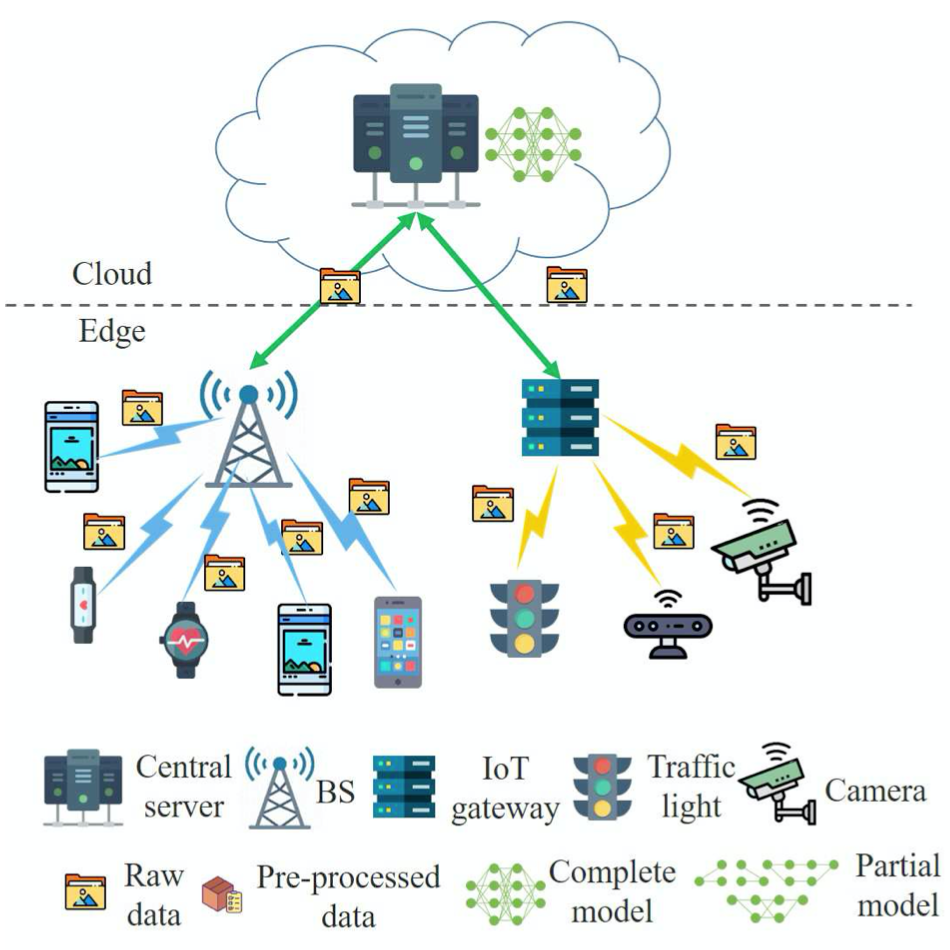
\includegraphics[width=10cm]{images/introduction/centralised_intelligence.png}
    \centering
    \caption{Centralised Intelligence}\label{fig:centralised_intelligence}
\end{figure}

In order to overcome to the above issues, a different approach is needed where
the data processing is not centralised but distributed closer where it is
generated: this different approach is called \textbf{edge computing},
Computing, storage and networking resources are located at the edge of the
network (IoT gateways, routers, etc\ldots) whilst end devices like mobile
phones and IoT devices request services from edge servers are called edge
devices.
It is easy to understand how this approach can address some of the issues in
the centralised intelligence: low latency between edge devices and edge servers
and data exchange and data privacy are some how mitigated.
It is worth noticing that edge computing is not a replacement for cloud
computing. On the contrary, it complements cloud computing and both are
targeting different kind of applications.

If we push a little more the design, the basis of edge computing combined with
AI creates what is called
\textbf{edge or mobile intelligence} (see~\ref{fig:edge_intelligence}).

This means that the data collection, caching, processing and analysis happens
on the device where the data is generated.
With this model latency, data privacy, network load and communication are all
contained and improved, giving a better experience to the end user and making
the application more reliable.

\begin{figure}[ht]
    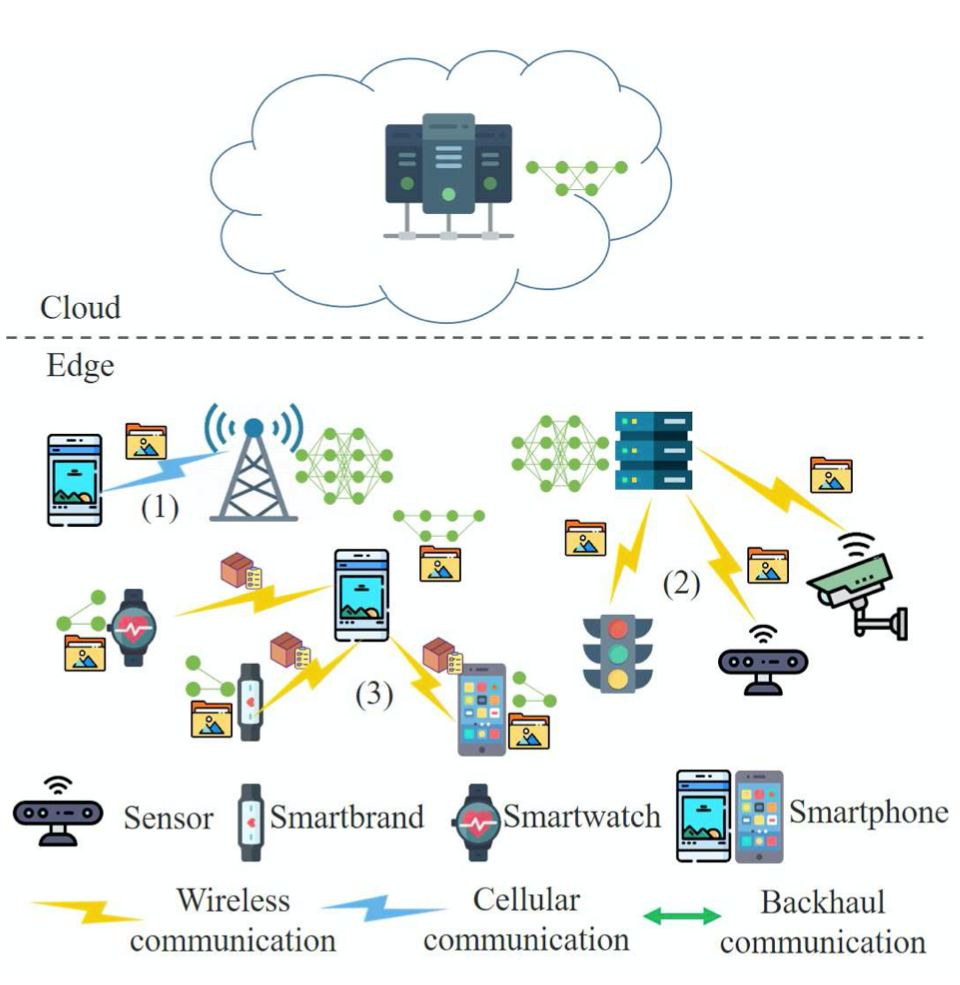
\includegraphics[width=10cm]{images/introduction/edge_intelligence.png}
    \centering
    \caption{Edge Intelligence}\label{fig:edge_intelligence}
\end{figure}

With more powerful end devices we start having edge intelligence applications
in our pockets like smart suggestions on the keyboards based on the context of
the text, photos application with integrated face recognition (note: no
personal data is sent to the cloud) based on contacts stored on the mobile and
voice recognition commands for offline translation and on mobile actions.~\cite{xu:2020}
Other examples are also self-driving cars, real-time applications and medical
devices but also noise cancellation on video call application like Microsoft
Teams. Interestingly enough, as counter example Google Meet uses its model on
the cloud leveraging Google TPU infrastructure.

In this thesis I focus mainly on the \textbf{edge inference} (~\ref{fig:edge_inference})
and specifically how the models can be optimised in order to reduce memory
footprint, size and compression without losing any accuracy in the prediction.

\begin{figure}[ht]
    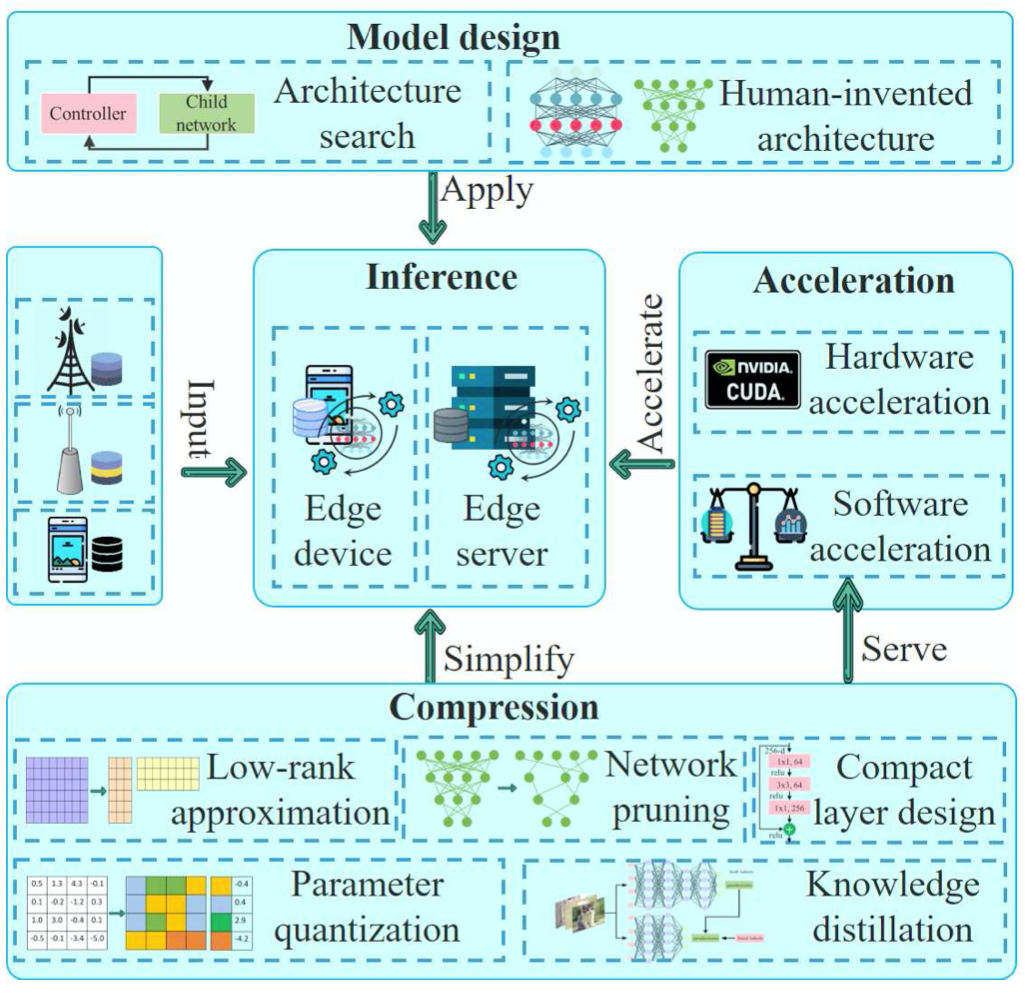
\includegraphics[width=10cm]{images/introduction/edge_inference.png}
    \centering
    \caption{Edge Inference}\label{fig:edge_inference}
\end{figure}

Edge inference is the final step of a model life cycle where the trained model
is used to infer new and unseen data via a forward pass of the neural network.
This step happens on the edge device and it presents some challenges due to the
limited amount of compute power and memory on the device itself.

In order to work correctly end efficiently the model needs to go through a
series of optimizations that decreases the power/memory consumption and latency
whilst maintaining the accuracy at acceptable levels \- ideally without
incurring in any decrease.

As the figure~\ref{fig:edge_inference} shows, there are different techniques
that it can be used to optimise models for edge inference. These are:
\begin{itemize}
    \item \textbf{Model design}: let the machines themselves design optimal
        models or human-invented architectures
    \item \textbf{Acceleration}: hardware acceleration mainly focus on parallel
        execution while software acceleration focuses on optimising resource
        management and compilers, based on compressed models
    \item \textbf{Compression}: low-rank approximation, knowledge distillation,
        compact layer design, network pruning and parameters quantisation are
        few techniques in order to achieve model compression
\end{itemize}

In this thesis I focus in a specific technique of model pruning.  In
\autoref{sec:training} I give an overview of the entire flow of an
intelligence application giving a brief explanation of every step of the flow.

In \autoref{sec:MO} I explain the main techniques for model optimization for
deployment, explaining what they are, pros and cons.

In \autoref{ch:pruning} I show the pruning technique more in details and
the section \autoref{sec:heuristic} illustrate the theory behind the per-layer
pruning configuration with heuristic.

In \autoref{ch:implementation} I show the code I have implemented in
TensorFlow Model Optimization giving full explanation and some working
examples.

Finally in \autoref{ch:results} I report experiment results on few well known
neural networks showing the benefits of this approach.

\section{From training to inference}\label{sec:training}

Pillars od edge intelligence: data, model and computation
Explain the whole flow
\lipsum[1]

\section{Model optimizations for deployment}\label{sec:MO}
* clustering
* quantization
* pruning
Pros and cons of each one following.
\lipsum[1]

\subsection{Clustering}
\lipsum[1]

\subsection{Quantization}
\lipsum[1]

\subsection{Pruning}
\lipsum[1]

\subsection{Combine multiple optimizations}
\lipsum[1]

Bibliographic citation